\documentclass[a4paper, 9pt, draft]{amsart}
\usepackage[english]{babel}
\usepackage{amsmath}
\usepackage{amssymb}
\usepackage{amsfonts}
\usepackage{mathtools}
\usepackage{diagbox}
\usepackage{booktabs}
\usepackage{enumitem}
\usepackage{color}
\usepackage{hyperref}
\usepackage{tikz}
\usepackage{accents}
\usepackage{standalone}
\usepackage{bm}
\usepackage{multicol}
\usepackage[font={small,sc}]{caption}

\usetikzlibrary{fit}
\usetikzlibrary{backgrounds}
\usetikzlibrary{positioning}
\usetikzlibrary{decorations}
\usetikzlibrary{decorations.pathmorphing}
\usetikzlibrary{arrows.meta}

\hyphenation{block-chain block-chains}

\hypersetup{colorlinks,
    citecolor=black,
    filecolor=black,
    linkcolor=black,
    urlcolor=blue,
    pdftex}

\setlist[description]{leftmargin=1.2cm, labelindent=\parindent}
\setlist[enumerate]{leftmargin=1.5cm, labelindent=\parindent}

\newcommand*\eg{e.g.\ }
\newcommand*\ie{i.e.\ }

\title[Oscoin]{Oscoin: Decentralized Code Collaboration}
\author{Monadic}
\date{2018}

\newcommand{\oscoin}{\textsc{\small{oscoin}}}
\newcommand{\blake}{\textsc{\small{blake2}}}
\newcommand{\hash}{\mathsc{hash}}
\newcommand{\coin}{$\Theta$}
\newcommand{\mathsc}[1]{\text{\normalfont\scshape#1}}
\newcommand{\tx}[2]{\langle \mathsc{#1}, #2 \rangle}
\newcommand{\tuple}[1]{\langle #1 \rangle}
\newcommand{\cvdots}{\multicolumn{1}{c}{\small{\vdots}}}
\newcommand{\dep}{\xrightharpoondown[e]{d}}
\newcommand{\notice}[1]{{\color{red}#1}}
\newcommand{\todo}{\notice{\texttt{TODO}}}

\newcommand{\rootchain}{\gamma}
\newcommand{\State}{\mathcal{S}}
\newcommand{\state}{\mathcal{S}}
\newcommand{\Ledger}{\mathcal{L}}
\newcommand{\Orgs}{\mathcal{O}}
\newcommand{\apply}{\Upsilon}
\newcommand{\fold}{\Upsilon}
\newcommand{\op}{T}

% Adjust spacing around equations. It can be a bit tight!
\expandafter\def\expandafter\normalsize\expandafter{%
    \normalsize%
    \addtolength{\abovedisplayskip}{2pt}%
    \addtolength{\abovedisplayshortskip}{2pt}%
    \addtolength{\belowdisplayskip}{2pt}%
    \addtolength{\belowdisplayshortskip}{2pt}%
}%

\newenvironment{fig}
  {\par\bigskip\noindent\minipage{\linewidth}}
  {\endminipage\par\bigskip}

% No paragraph indentation after section headers.
\makeatletter
\let\@afterindenttrue\@afterindentfalse
\makeatother

% Issue amend operator.
\DeclareMathOperator{\amend}{\times}

\newenvironment{epigraph}[2][]
{\leftskip=1cm \def\epigraph@author{#2} \smallskip\itshape}
{\par\vspace{0.5em}\normalfont\hfill---\ \epigraph@author\hspace*{0.2cm}\par\medskip}
\makeatother

\setlength{\textwidth}{\paperwidth}
\addtolength{\textwidth}{-4cm}
\setlength{\textheight}{\paperheight}
\addtolength{\textheight}{-5cm}
\calclayout

\begin{document}
\begin{abstract}
    Over the last few decades, with the emergence of open-source software,
    we've experienced an unprecedented acceleration in the development of our
    digital infrastructure, one that has become a new commons -- a public good
    we are now collectively responsible for. But we are all familiar with cases
    like Heartbleed, with developer burn-out, with projects acquired by
    ill-incentivized or incompetent parties. Today, many valuable open-source
    software projects are unable to define themselves in traditional market
    terms, while others find it incompatible with their ethics and struggle
    without financial support. Oscoin is a proposed solution to this problem
    which leverages technology and mechanisms pioneered by early
    crypto-currencies such as Bitcoin and Ethereum.  In a network based
    economy, value should be distributed transparently towards the members who
    contribute value to the network, instead of being captured by a few.  We
    believe that crypto-economies are a means of creating financially
    sustainable decentralized communities.
\end{abstract}
\maketitle

\setlength{\columnsep}{20pt}
\begin{multicols}{2}

\section{Introduction}
\label{s:introduction}

% Replicated state machines. Examples (Paxos, blockchains, etc.). It's purpose
% and constraints

% Variety of applications. Is there a unifying abstraction? Needs to be
% deterministic, but aside from that, a DSL-language.

% Mention radicle.

% Allows for updates that benefit from the same consistency guarantees as the
% operations themselves. Helps solve the problem of software updates in Paxos
% etc, and a more powerful form of self-amendment in blockchains. [Note that
% perfomance gains in the compiler/interpreter must happen differently, though
% separating changes that can be semantic from those that are not helps.]

% Effect system. Separating out impurity. In the case of blockchains, clients
% are *also* programmable, without sacrificing consensus.

% outline.
% Section 2) Some examples: an upgradable key-value store. A version of nomic.
% Section 3) Formal description of language.

Replicated state machines are a widely used paradigm to program fault-tolerant
systems. The paradigm involves deploying a deterministic state machine across
multiple nodes (servers); these nodes can respond to client requests, and by
agreeing on the order of these requests (consensus), ensure agreement on their
state and output. If some fraction of nodes is unavailable (or in the looser
requirement of blockchains, if they are malicious), the overall system can
still function correctly.

The service these systems replicate may be key-value stores, file-systems,
append-only logs, account balances, etc. Each of these
services is often re-implemented anew, leading to substantial development
costs, as well as subtle bugs in the interim state of the system during the
inevitable software upgrades. In this paper, we describe a language, \rad, for
defining the behaviour of replicated state machines (RSMs) independently of the
underlying consensus. The language is designed so that new domain-specific
languages (DSLs) can easily be defined for each service provided by the system.
Each such DSL is the definition of an RSM. The expressions of the DSL
are the RSMs inputs; the value such an expression evaluates to its outputs; and
the changes in the environment its state changes.

Thus, if for example the RSM we are interested
in is a ledger of accounts, expressions or inputs may be transfers, the
state may be the balance and ownership of accounts, and outputs may be the new
balances of affected accounts or an error message if the transfers are not
allowed (due to insufficient funds or incorrect permissions).

Additionally, using the same mechanism as for DSL-definition (namely, a
\emph{reflective tower}), we provide a way for upgrading the DSL itself
\emph{with the same guarantees of agreement} between nodes as the underlying
consensus, reducing the coordination difficulty of an upgrade. DSLs can be
defined in such a way that \emph{re}-definitions are themselves just one of the
sorts of inputs RSM accepts; thus nodes will agree on the ordering of the
upgrade with respect to other inputs, and will not go out of sync as a
consequence of update.

While (crucially for the purpose of ensuring consensus) the core of the language
is deterministic, \rad also possesses an additional set of primitive operations
that allow side-effects. We show how a publish-subscribe model for side-effects
(or in the formalism of \cite{Cartwright1994}, an effect-handling central which
is never provided continuations) allows responding to outputs of the state
machine or state changes in a non-deterministic way, without endangering the
determism of the state machine itself. This in turn makes the separation between
reads and writes correct by construction.

\rad has been developed in the context of a broader effort to create a
community-owned platform for open-source development (\oscoin{}), which
includes a consensus algorithm and a networking component. The \oscoin{}
platform allows users and communities to create permissioned and permissionless
RSMs with their own semantics, be it to maintain decentralized
version-controled code, issues, pull requests, or collective decision-making. \rad is
oriented towards making that process as simple and clear as possible. We do
not in this paper further discuss the broader \oscoin{} system.

In the rest of the paper, we show some example applications built with
\rad---first, an upgradable key-value store, and then more ambitiously, a game
of Nomic (Section \ref{s:examples}). We then describe the language in more
detail (Section \ref{s:language}), and compare it to other technologies.

\section{Core Architecture}
\label{s:core-architecture}

% TODO: Reference Tezos.
% TODO: Reference Holochain.
% TODO: Reference Snowflake?
% TODO: Reference Scuttlebut.

In order to represent partial as well as totally ordered operations over the
network, \oscoin{} employs a DAG-like data-structure which we shall refer to as
the ``block-tree''.  Our block-tree starts from a \emph{root} chain and splits
into sub-chains via a process called branching. We thus refer to the sub-chains as
\emph{branches}.  Operations on the tree are represented by cryptographically
linked blocks of transactions (``blockchains''), with the most recent block in
any given branch known as the tip of the branch, or \emph{leaf}.

This design affords us several advantages over traditional blockchains, namely
the freedom to incorporate partially-ordered transactions within the semantics
of the protocol, as well as the ability to define semantics on a per-chain
basis, as we shall see in \S~\ref{fold-function}.

\todo{Motivate this architecture better?}

% TODO: Motivate. Basically, same thesis as Tezos, but
% done differently, with code on-chain. Also allows governance to change
% validation functions, which you can't do otherwise.
% Mimics the branching model of VCSs.

% * Partial ordering
% * Self-amending
%   * Governance (code on-chain)
%   * Protocol upgrade (semantics only)
% * Single writer
%   * Instant-finality
%   * Offline capable
%   * Agent-based
% * Scalability
%   * Logical sharding
%   * Selective syncing (following)

\subsection{Overview}

The first block of any chain is called the \emph{genesis}. We represent a chain
$C$ as a sequence of blocks $B_0 \dots B_h$ where $B_0$ is the genesis,
$B_h$ is the leaf, and $h$ is the height of $C$. Within the genesis, the
semantics of a chain is defined by an initial state $S_0$ known as the
genesis state. The state of all chains is collectively known as the root state
$\state$ which represents a hierarchy of states starting from the root
and descending into the state of each branch.

\subsection{State}

The state $S$ of a chain can be defined as a function mapping a key $k \in K$ to a
value $v$. We define the special form $S[k]$ as:
\[
    S[k] \equiv \begin{cases}
        v                   & \text{if} \quad k \in K \\
        \bot                & \text{otherwise}
    \end{cases}
\]

\subsection{The $\fold$ Function} \label{fold-function}

Within its target set, $S$ contains a value $S[\fold]$ or more succinctly
$\fold$ which describes how $S$ is to be interpreted. This recursive definition
of $S$ and $\fold$ is key to implementing a self-describing and self-amending
chain. Formally, we define $\fold$ as a function
\[
    \fold : (\env, t) \mapsto \env',
\]
where $\env$ is a given execution environment, $t$ is an operation to be
evaluated within that environment, and $\env'$ is the resulting environment
after applying $\fold$.  In the context of a chain $C$, we can say that $\env
\equiv S$ and describe the state $S_{h+1}$ of $C$ after applying a
sequence of transactions $t_1 \dots t_n$ as the recursive application of $\fold$:
\[
    S_{h+1} \equiv \apply(\cdots \apply(\apply(\apply(S_h,
    t_1), t_2), t_3) \cdots t_n).
\]

Since $\fold$ is defined within $S$ as $S[\fold]$, $\fold$ is also
able to amend itself as part of this state transition, and so we can say that:
\[
    \exists t \in \mathcal{T} : \fold(S, t)[\fold] \neq \fold,
\]
where $\mathcal{T}$ is the set of transactions recognized by $\fold$.  Note
that $t$ is not defined as part of the base protocol. Instead $t$ is
interpreted by the fold function $\fold$, and its semantics entirely determined
by it. This gives $\fold$ complete flexibility, as we shall see in
\S~\ref{s:root}.

\subsection{The Block-Tree}

So far we've talked about single chains with a state $S$ and fold function
$\fold$, but our architecture notably allows chains to form a tree structure,
via \emph{branching}. This ``block-tree'' is represented formally as a set
$\tree$ of chains, where every chain $C \in \tree$ is either the parent of a
chain, its descendant, or a sibling. When a chain $C'$ branches off its parent
chain $C$, we denote this as $C \prec C'$.

Though there is a clear hierarchy between the branches, blocks are allowed to
refer to an arbitrary number of parents, making the ``block-tree'' exhibit the
properties of a DAG.

\todo{Transition.}

\subsubsection{The Root and Radicle}
\label{s:root}

In the beginning, we have only one chain, known as the \emph{root}, with a
single block, the \emph{radicle}. This initial state, which is effectively the
genesis of the first chain is the ancestor of all branches, and is the only
block with no parent.

Besides having no parent, the radicle is special in that it is applied to the
genesis root state $\state_0$ by the genesis fold $\fold_{0}$. This particular
fold is defined as:
\[
    \fold_{0} \equiv (\env, t) \mapsto \eval (\env, t),
\]
or more succinctly,
\[
    \fold_0 \equiv \eval,
\]
where $\eval$ is the \emph{eval} function of some interpreted language $L$.
Thus, at genesis, $t$ can be any valid expression in $L$, effectively giving
the root chain the properties of a read-eval loop, where the resulting
environment after evaluation is carried to the next block.

\todo{Something about "This programming environment can be used to..."} \\
\todo{Reference lisp/scheme?} \\
\todo{read-eval-commit loop?}

\subsubsection{Branching}

In every block header there is what we call a \emph{chain-id}. This identifier,
formally $H_{id}$ is used by the protocol to understand the intent of a block;
to decide what to do with it in the case where more than one block exists with
the same parent hash.

Let $A$, $B$ and $B'$ be blocks considered by the protocol where $A \prec B
\wedge A \prec B'$.  Let $b$ be the chain-id of $B$,  $b'$ be the chain-id of
$B'$, $a$ be the chain-id of $A$, and $b \neq b'$. There are two scenarios
that come to play assuming only valid blocks.

\begin{enumerate}
    \item If $b = a$ and $b' = a$, then $B$ and $B'$ are in \emph{conflict}.
        This means only one of the two will be chosen to succeed $A$. To
        resolve this, the protocol uses the \textsc{score} function discussed
        in \S~\ref{consensus} to decide which block to build upon.
    \item If $b \neq a$ or $b' \neq a$, then we have a \emph{branch}. The block
        or blocks which do not have a matching chain-id with their parent $A$
        will consistute a new chain with new chain-id. This new chain will
        exist alongside $A$'s chain, and will share an ancestry or ``prefix''
        with $A$.
\end{enumerate}

This simple rule means that the only difference between a chain and its branches
is the chain-id, and to create a branch, one needs only to submit a block with
a unique chain-id.

\todo{Talk about following chains.} \\
\todo{Talk about having to read chains all the way up to the ancestor's genesis.} \\
\todo{As you go up, the chain-id changes because all chains except the root are branches.} \\
\todo{Another way to follow a chain is to start from a leaf and follow it up to its genesis.}

% TODO: Diagram for this ^


\section{Seed Protocol Semantics}
\label{sec:protocol-semantics}

% TODO: Distinguish operations from messages, make sure messages aren't signed.
% TODO: Make sure all operations, ex. around issues are using a message token.

With the core architecture out of the way, we can now describe the \oscoin{}
seed protocol in terms of $\fold$ and $\state$. Since the protocol is amendable
due to our definition of $\fold$, we define a \emph{seed} protocol, which has
the ability to evolve based on its user's needs.

The rules according to which transactions on the \oscoin{} network are
validated comprise a \emph{protocol}. This protocol has a well defined semantics
which we shall describe in this section.

\subsection{Overview} The \oscoin{} protocol is composed of interrelated
\emph{objects} which form a hierarchical graph as seen in Figure
\ref{object-relationships}, and \emph{operations}, which act on these objects.

\medskip

\begin{fig}
\centering
\begin{tikzpicture}[sibling distance=8em]
    \node {\emph{root}}
        child { node {\emph{tokens}} }
        child { node {\emph{accounts}}
            child { node {\emph{keys}} }
            child { node {\emph{repositories}}
                child { node {\emph{patches}} }
                child { node {\emph{proposals}}
                    child { node {\emph{patchset}} }
                    child { node {\emph{votes}} } } } };
\end{tikzpicture}
\bigskip
\captionof{figure}{Object hierarchy in the \oscoin{} protocol.
\label{object-relationships}}
\end{fig}

\subsection{The Root}
In the beginning, we have only one chain, known as the \emph{root}. In its simplest
form, the genesis of the root chain would be defined as an empty state $\varnothing$
and a fold function $f$ which allows only one operation called $branch$, which takes
an identifier, a fold function of its own and creates a branch with the given
fold function as $\fold$.

\subsection{Operations and State}
\label{operations-and-state}

% TODO: Call operation messages 'commands'. Then refer to all future
% operations as commands. Move the author, nonce etc. to the command. Make
% operations as a sequence of commands.

% TODO: Better word for Contexts?
% TODO: Issue resolution. Voicing. Voicing can be used to implement voting mechanisms.
% TODO: Merge accounts (A) and orgs (O).
% TODO: Change apply function to *fold* function.

Operations are signed messages constructed by participants in the protocol,
which trigger a state transition in the network. An operation $\op$ takes
the form:
\[
    \op \equiv \tuple{\op_i, \op_m, \op_p, \op_n}_{\sigma}
\]
where $\op_i$ is the identity of the sender of the operation, $\op_m$ is the
message, $\op_p$ is a reference to a parent operation, such that $\op_p \prec
\op$. Finally, $\op_n \in \mathbb{N}$ taken together with $\op_i$ forms a
globally unique operation identifier, such that there can be at most one
operation with a given $\tuple{\op_i, \op_n}$ tuple. If $\mathcal{T}$ is the
set of all operations, then $\mathcal{T}_v \subset \mathcal{T}$ is the set of all \emph{valid}
operations.

An operation $t \in \mathcal{T}_v$ applied to the current state of the protocol $\mathcal{S}_e$
at epoch $e$ can be formulated as:
\[
    \mathcal{S}_{e+1} \equiv \apply(\mathcal{S}_e, t)
\]
where $\apply$ is the state-transition function defined by:
\[
    \apply(\State, t) \equiv \begin{cases}
        \apply_{s}(\State, t) & \text{if} \quad t \in \mathcal{T}_v \\
        \State                & \text{otherwise}
    \end{cases}
\]
and $\apply_s$ is a sub-function of $\apply$ which applies valid operations to
$\State$.  We can describe the current
state of the network $\mathcal{S}_e$ as a sequence of operations $\mathcal{L} =
\op_1 \dotso \op_e$, (the ``ledger'') applied recursively to an initial empty
state $\varnothing$:
\[
    \mathcal{S}_e \equiv \apply(\dotso \apply(\apply(\apply(\varnothing,
    \op_1), \op_2), \op_3) \dotso \op_e)
\]
The state $\mathcal{S}$ of the protocol is defined as:
\[
    \mathcal{S} \equiv \tuple{\mathcal{A}, \mathcal{O}, \mathcal{D}, \mathcal{C}, \mathcal{L}} \\
\]
where $\mathcal{A}$ is the set of accounts (\S \ref{accounts}), $\mathcal{O}$
is the set of organizations known to the protocol (\S \ref{orgs}),
$\mathcal{D}$ is the set of dependencies between projects (\S
\ref{dependencies}), $\mathcal{C}$ is the set of contexts onto which patches
can be applied (\S \ref{contexts}) and $\mathcal{L}$ is the sequence of
operations which have been applied to $\mathcal{S}$. It is thus possible to
reconstruct $\mathcal{S}$ from $\mathcal{L}$ via the $\apply$ function, as
seen above. In the remainder of the section, we shall use the word
\emph{operation} to mean a valid message that has been applied to the state
$\State$ and recorded in a ledger $\Ledger$, and \emph{message} to mean an
object sent between participants of the protocol to communicate.

\subsection{Patches}
\label{patches}

The fundamental product or \emph{artifact} of the \oscoin{} network is code, or
source code. Our protocol defines the \emph{patch} primitive as the atomic unit
of code. A patch is a set of metadata and code changes, or \emph{changeset},
that can be applied to an existing body of code, or \emph{context}, to modify
it. We define a patch $P$ as the tuple $\tuple{P_i, P_m, P_f}$, where $P_i$ is
the identity of the author of the patch, $P_m$ is the patch metadata and $P_f$
is the changeset. A set of patches in no particular order is called a
\emph{patchset}.

Patches can be composed sequentially, taking an initial context $A$ into
a modified context $B$. The empty context is defined as $\varnothing$, such
that there exists a mapping $P_f \varnothing \mapsto P_f$. Let $f \prec g
\prec h$ be an ordered sequence of patches, then the formulation:
\[
    h \cdot g \cdot f : A \to B
\]
is the in-order composition of patches $f$, $g$ and $h$, taking an initial
context from $A$ to $B$. In \oscoin{}, typical examples of contexts include
code repositories, files and branches.

% TODO: Repository section. A repository is a context C, initially {} with an
% identifier (to which patches can refer), that patches can be applied to,
% and issues can refer to.

% TODO: In git, a repository contains: a set of commit objects, a set of
% references called 'heads', to commit objects (ex. branches).
% A project always has one commit object with no parents, this is the first
% commit.

% TODO: Storing patch metadata (instead of hash, and not the changeset) is for
% 'lazy-repositories' - you can download them and read the history without
% downloading the files.

% TODO: The sequence of patches is called the 'inventory'. Doesn't seem to have
% parent pointers in darcs!

% TODO: There's a "set of patches" and a "sequence of patches". They are both
% useful views on the dataset.

% "any permutation of a patch sequence allowed by Darcs leads to the same exact repository (if not, we have a bug)" ?!
% TODO: Therefore there is a set of valid orders which lead to the same repository!

\subsubsection{The \textsc{patch} message}
\label{patch-op}

To exchange patches amongst protocol participants, we define the
$\tx{patch}{p}$ message, which allows a patch or patchset $p$ to be broadcast
to all participants.

\subsubsection{The \textsc{record} message}
\label{record-op}

In order for a patch or patchset to be applied to some context $r_c \in
\mathcal{C}$ , we define a message $\tx{record}{r_p, r_c}$, which takes a
patchset $r_p$ and applies it to a context $r_c$.

\subsubsection{The \textsc{fork} message}
\label{fork-op}

Given an existing context $k_c$, the $\tx{fork}{k_c, k_{c'}}$ message derives
a new context $k_{c'}$ which shares all existing patches with $k_c$. From that
point on, $k_c$ and $k_{c'}$ are allowed to diverge.

The \textsc{fork} message can also be used to create entirely new contexts, by
passing the empty context $\mathcal{C}_\varnothing$ as $k_c$.

\subsection{Contexts}
\todo{}
% TODO: (Account, {Repo, File, ...})

% TODO: Concept of ownership!?

% TODO: Are patches tied to orgs/repos/branches, or free-floating, and the
% PATCH operation is what is tied to them?


% TODO: Contexts form a free monoid?
% TODO: Reference patch theory.

\subsection{Issues}
\label{issues}

On the \oscoin{} network, collaboration on code takes place through \emph{issues};
and since project governance is specified in code---through the use of
\emph{smart contracts}---organizational decisions are also made through issues.

% TODO: Remove reference to smart contracts!

An issue $I$ is described at epoch $e$ by the tuple:
\[
    \big<\tuple{I_a, I_t, I_b, I_o, I_r, I_P}_{\sigma}, I_s, I_V \big>_e
\]
where $I_a$ is the issue author, $I_t$ is the title or subject of the issue,
$I_b$ is the description in plain text of the issue, $I_o$ is a list of
operations to be applied when $I_s$ changes, $I_r$ is the issue resolution
function, $I_P$ is the patchset attached to the issue, $\sigma$ is the
signature of $I_a$, $I_s \in \{open, closed, accepted, rejected\}$ is the
current state of the issue and $I_V$ is the set of votes on the issue. The
initial value of $I_s$, $I_{s_0} = open$, the initial value of $I_V$, $I_{V_0}
= \varnothing$ and the initial value of $I_P$, $I_{P_0} = \varnothing$.  The list
of valid state transitions between any two states $I_s$ and $I_{s'}$ are as
follows:

\begin{fig}
    \centering
    \captionof{table}{Valid state transitions.\label{issues-valid-transitions}}
    \begin{tabular}{@{}rcl@{}}
        \toprule
        $I_s$      & $\to$ & $I_{s'}$ \\
        \midrule
        $open$     & $\to$ & $accepted$ \\
        $open$     & $\to$ & $rejected$ \\
        $open$     & $\to$ & $closed$ \\
        $closed$   & $\to$ & $open$ \\
        \bottomrule
    \end{tabular}
\end{fig}

The patchset $I_P$ attached to an issue represents a set of proposed changes to
some project, while the subject $I_t$ and body $I_b$ of the issue provide a
description of the changes contained in $I_P$. Issue \emph{resolution} is the
process of voting on an issue with the aim to move to an \emph{accepted} or
\emph{rejected} state.

Issues can be voted on with the \textsc{voice} operation. When an issue receives
a new vote, it is added to $I_V$. A vote $v$ is represented by the tuple
$\tuple{v_i, v_a, v_{\omega}, v_e}_{\sigma}$ where $v_a$ is the voter,
$v_i$ is the issue being voted on, $v_{\omega} \in \{accept, reject\}$ and
$v_e$ is the epoch $e$ at which the vote is valid.

When a certain threshold of votes is reached, an issue transitions to either an
\emph{accepted} or \emph{rejected} state. Given an open issue $i$, the rules of
issue resolution are defined by the function $i_r : I \to I$, applied to the
issue $i$ for every vote added to $i_V$.

\subsubsection{Amendments}

An issue $I$ where $I_s = open$ can be amended with the \textsc{amend}
operation, or $\amend$. Only $I_t$, $I_b$, $I_o$, $I_r$ and $I_P$ can be
amended.  Amending an issue creates a new empty set of votes $V'$, ensuring two
versions of a given issue never share a set of votes. Formally, amendment is
defined as:
\begin{align*}
    I \amend{} \langle I_a, t', b', o', r', P' \rangle_{\sigma} \equiv
    \big<\langle I_a, t', b', o', r', P' \rangle_{\sigma}, I_s, \varnothing
    \big>
\end{align*}
where $I_s = open$.

% TODO: The amendment should include the issue it is amending.

\subsubsection{Accepted Issues} When an issue has been accepted by a majority
of votes, the issue transitions permanently into an \emph{accepted} state. The
steps taken by the protocol are as follows:

\begin{enumerate}
    \item The issue's state $I_s$ is set to \emph{accepted}.
    \item The issue is \emph{frozen}, such that no further amendments or state
        changes are possible.
    \item The list of operations $I_o$ belonging to the issue are executed by
        the protocol.
    \item The issue's \emph{patchset} $I_P$ is permanently added to the code
        project it pertains to. Note that a patchset may contain individual
        patches pertaining to different projects, in which case the patches are
        applied individually to their respective projects.
\end{enumerate}

\subsubsection{Rejected issues} When an issue is rejected,
\begin{enumerate}
    \item The issue transitions to a \emph{rejected} state.
    \item The issue is frozen so that no further amendments or state
        transitions are possible.
    \item The list of operations $I_o$ belonging to the issue are executed by
        the protocol.
\end{enumerate}

\subsubsection{Closed issues} When an issue is closed, its state changes to
\emph{closed} until it is re-opened. No operations from $I_o$ are run, since
an issue can be opened and closed many times. Only the author $I_a$ of an issue
can close it.

\subsection{Value}

To enable the transfer of value in the network, the protocol defines a scarce
currency we shall refer to in the remainder of this paper as~\coin{}, or
\oscoin{}.

\subsubsection{Supply}

The supply of \coin{} is subject to an inflation $e_{\iota} \in \mathbb{N}$,
carried out by the protocol every epoch $e$, and determined by a logarithmic
function $f : e \to e_{\iota}$, such that $\lim_{e \to \infty} f(e) = 0$.

\subsubsection{Accounts}
\label{accounts}

Currency is held in \emph{accounts} which can be unlocked by the signature of
the account holder. Accounts have addresses which are used to send and receive
\coin{}. The set of all accounts is known as $\mathcal{A}$.

\subsubsection{Transfer}

Value can be transfered from one account to another with the \textsc{send}
message, formally defined as $\tx{send}{a_{s}, a_{r}, n}$, where $a_{s}$ and
$a_{r}$ are the \emph{sender} and \emph{recipient} addresses between which the
value should be transfered and $n$ is the value to transfer.  To be valid, a
\textsc{send} operation must be signed by the owner of $a_{s}$.

\subsubsection{Bonding}

Value can be locked in the system via an operation called \emph{bonding}.
This operation turns \emph{liquid} value into \emph{bonded} value, preventing
them from being moved for a certain amount of time, and can be used to perform
security deposits or other forms of commitment which require a collateral or
pledge. Bonding and unbonding operations are performed with the
\textsc{bond} and \textsc{unbond} messages defined as:
\[
    \tx{bond}{a, a_b, n} \qquad \tx{unbond}{a, a_b, n}
    \medskip
\]
where $a$ is the address from which to withdraw the value for bonding, $a_b$ is
the address where the value is to be bonded and $n$ is the value to bond. When
the \textsc{unbond} operation is used, an unbonding period $e_u$ is started,
measured in epochs. Once $e_{u}$ epochs have passed, the value is withdrawn
from the bonding address $a_b$ and credited back to $a$.

\subsection{Organizations}
\label{orgs}

An organization $O$ is described by the tuple:
\[
    \tuple{O_{id}, O_{a}, O_R, O_M}
\]
where $O_{id}$ is the organization's identifier, $O_a$ is its account, $O_R$ is
the set of repositories under $O$ and $O_M$ is the set of members belonging to
the organization. We can relate patches (\ref{patches}) and issues
(\ref{issues}) to repositories with the equations:
\begin{align*}
    O_R & \equiv \{R_1, R_2, \dotsc, R_n\}         \\
    R   & \equiv \tuple{R_{id}, R_I, R_P}         \\
    R_I & \equiv \{I_1, I_2, \dotsc, I_n\}         \\
    R_P & \equiv \tuple{P_1, P_2, \dotsc, P_n}
\end{align*}
where $R_{id}$ is the repository's identifier, $R_I$ is the set of issues
related to $R$, and $R_P$ is the sequence of patches composing its codebase.

The set $\mathcal{O} = \{O_1, O_2, \dotsc, O_n\}$ is the set of all organizations
known to the protocol.  Let $o$ be an organization, then $\tx{register}{o}$ is
an operation that registers $o$ and makes it known to the protocol such that:
\[
    \apply_o(\mathcal{O}, \tx{register}{o})
    \equiv \mathcal{O} \cup \{o\}
\]
where $\apply_o$ is a sub-function of $\apply$, and defines
state-transitions in $\mathcal{O}$.

\subsection{Dependencies}
\label{dependencies}

A project $a$ depends on a project $b$ at epoch $e$ if it references $b$
or parts of $b$. Formally, we represent this as:
\[
    D \equiv \tuple{D_a, D_b, D_e} \qquad \text{or} \qquad a \dep b
\]

% TODO: dependencies with \overrightarrow{AB}, like vectors.

Let $R^*$ be the set $O_{1_R} \cup O_{2_R} \cup \cdots \cup
O_{n_R}$ of all projects across all organizations, and $\mathcal{D}_e$ be the
set of all dependencies at epoch $e$, then:
\[
    \mathcal{D}_e \equiv \{(a, b) : a \in R^*
    \land b \in R^*
    \land a \dep b \}
\]

Dependencies are recorded with the
\[
    \tx{depend}{D_a, D_b, D_e, D_{e'}}
\]
operation, which records a dependency between $a$ and $b$ for each epoch $x$
where $e \leqslant x \leqslant e'$.

\section{Network Protocol and Architecture}

The \oscoin{} network protocol is a realization of the protocol semantics
described in \S~\ref{sec:protocol-semantics}, into the asynchronous network
model.

\subsection{Overview}

The \oscoin{} network is composed of a set of nodes, or \emph{replicas}, which
execute a protocol $\mathcal{P}$. Together, these nodes form a \emph{Replicated
State Machine} with a set of states $\State^*$, a transition function $\apply$,
a starting state $\State_0$, a set of inputs $B_0 \dotso B_n$, and an empty set
of outputs.

% TODO: Are we using the 'P' variable?

Participation in the network protocol is \emph{open} (\ie ``permissionless''),
which makes the replica set dynamic. To achieve consensus in the permissionless
setting, we make use of blockchains~\cite{bitcoin} as the underlying replicated
data-structure, with a method of Sybil resistance such as proof-of-work or
proof-of-stake.  However, unlike other blockchain protocols, we describe a
multi-chain ``block-lattice'' \cite{raiblocks} design with causal consistency
guarantees \cite{causal-consistency} and partial ordering across chains
(Figure~\ref{block-lattice}).

The \oscoin{} protocol can be paired with any blockchain consensus algorithm,
given certain requirements discussed in \S~\ref{consensus}.

\subsection{Block-lattice Architecture}

Block-lattices are a replicated data-structure composed of chains of blocks,
depicted in Figure~\ref{block-lattice}.  Both parallel and synchronized
operations are able to be expressed with this design:  a pair of transactions
on two chains are considered \emph{free}, if they may be processed in parallel,
or \emph{dependent}, if a causal or acausal dependency exists between them.

Each chain in our design functions as a logical unit of organization,
governance, and funding. In other words, each user, organization or community
is expected to operate under their own chain. These individual chains are
called \emph{accounts}. The block-lattice design has numerous advantages for
our use case, including parallel transaction processing, minimal resource
requirements for light clients, instant finality for certain kinds of
transactions, and logical sharding at the account level.

\begin{figure*}[!ht]
    \documentclass[tikz]{standalone}

\usetikzlibrary{fit}
\usetikzlibrary{positioning}

\begin{document}
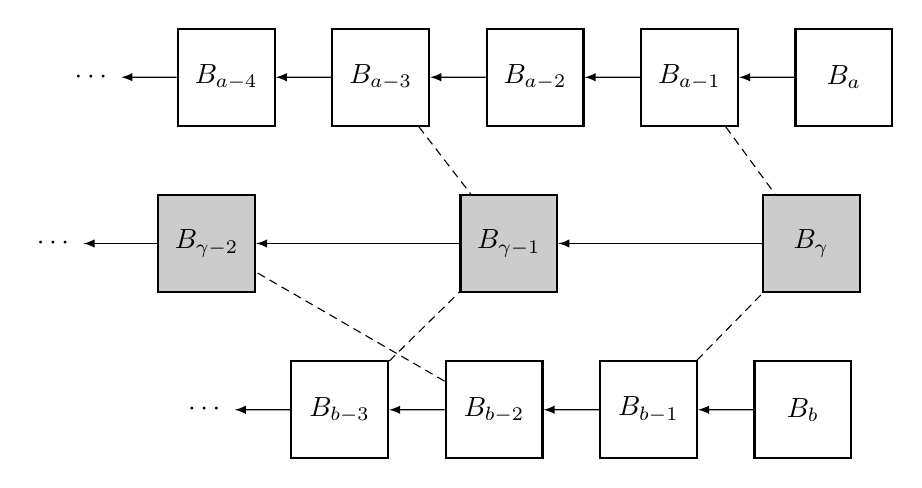
\begin{tikzpicture}[scale=0.96]
    \tikzstyle{root} = [draw=black, thick, fill=black!20, rectangle, minimum height=3.5em, minimum width=3.5em, node distance=3em];
    \tikzstyle{org-block} = [draw, thick, fill=white, rectangle, minimum height=3.5em, minimum width=3.5em, node distance=2em];
    \tikzstyle{link} = [-, thin, densely dashed];
    \tikzstyle{pointer} = [thin, -latex];

    \node (org-a-0) at (-2.5, 2.2)                {$\cdots$};
    \node[org-block] (org-a-1) [right=of org-a-0] {$B_{a-4}$}
        edge [pointer] (org-a-0.east);
    \node[org-block] (org-a-2)  [right=of org-a-1] {$B_{a-3}$}
        edge [pointer] (org-a-1.east);
    \node[org-block] (org-a-3)  [right=of org-a-2] {$B_{a-2}$}
        edge [pointer] (org-a-2.east);
    \node[org-block] (org-a-4)  [right=of org-a-3] {$B_{a-1}$}
        edge [pointer] (org-a-3.east);
    \node[org-block] (org-a-5)  [right=of org-a-4] {$B_{a}$}
        edge [pointer] (org-a-4.east);

    \node (root-0) at (-3, 0)        {$\cdots$};
    \node (root-1) at (-1, 0) [root] {$B_{\rootchain - 2}$}
        edge [pointer] (root-0.east);
    \node (root-2) at ( 3, 0) [root] {$B_{\rootchain - 1}$}
        edge [pointer] (root-1.east);
    \node (root-3) at ( 7, 0) [root] {$B_{\rootchain}$}
        edge [pointer] (root-2.east);

    \node (org-b-0) at (-1, -2.2) {$\cdots$};
    \node[org-block] (org-b-1) [right=of org-b-0] {$B_{b-3}$}
        edge [pointer] (org-b-0.east);
    \node[org-block] (org-b-2) [right=of org-b-1] {$B_{b-2}$}
        edge [pointer] (org-b-1.east);
    \node[org-block] (org-b-3) [right=of org-b-2] {$B_{b-1}$}
        edge [pointer] (org-b-2.east);
    \node[org-block] (org-b-4) [right=of org-b-3] {$B_{b}$}
        edge [pointer] (org-b-3.east);

    \draw [link] (org-a-2) -- (root-2);
    \draw [link] (org-a-4) -- (root-3);
    \draw [link] (org-b-2) -- (root-1);
    \draw [link] (org-b-1) -- (root-2);
    \draw [link] (org-b-3) -- (root-3);
\end{tikzpicture}
\end{document}

    \caption{Block-lattice design. $B_a$, $B_b$ and $B_c$ are chains partially ordered in relation to one another.\label{block-lattice}}
\end{figure*}

\subsection{Threat Model}

We assume a majority ($> 50\%$) of honest, or \emph{compliant} nodes which follow
the protocol. In other words, for $f$ non-compliant (faulty) nodes, we assume a
network of $2f+1$ nodes in total.

\subsection{Blocks, State and Transactions}

In \S~\ref{operations-and-state}, we saw that the protocol semantics could
be defined in terms of a global state $\State$ and a sequence of operations
$\op_1 \dotso \op_n$ applied to $\State$, forming a ledger $\Ledger$. When
describing the network architecture and protocol, a direct mapping between
these abstract objects and the components of the software architecture exist.

\subsubsection{State}

The state $\State$ is represented by a function $\State : K \to V$ which maps a
set of keys $K \in \mathbb{B}^{256}$ to a set of values $V \in \mathbb{B}^{*}$,
where $\mathbb{B}$ is the set of bytes, and $\mathbb{B}^n$ is the set of byte
strings of length $n$. The initial state $\State_0$ is called the
\emph{genesis} state. Since we are working with multiple chains, and each
chain represents an account's ledger, we define $\mathcal{A}_i$ to be the state
of account $i$ and $\mathcal{L}_i$ to be $i$'s ledger.

\subsubsection{Block}

An operation $\op$ is represented by a sequence of one or more transactions,
organized in a \emph{block}. A ledger $\Ledger$ of all valid recorded
operations is represented as a sequence of blocks, or \emph{blockchain}. A
block $B$ in \oscoin{} consists of a block header $B_H$ with a set of fields
(Table~\ref{block-header-fields}.) and a sequence of transactions $B_T = (t_0
\dotso t_n)$.

% TODO: Is it zero or more txns?

\begin{table*}[htp]
    \caption{Block header fields \label{block-header-fields}}
    \begin{tabular}{l c p{7.5cm}}
        \toprule
        Field                  & Notation & Description \\
        \midrule
        \emph{Chain}           & $H_{id}$ & The name or identifier of the chain, \eg ``oscoin.'' \\
        \emph{Height}          & $H_n$    & The block height. \\
        \emph{ParentHash}      & $H_p$    & The \blake{} hash of the parent block header. \\
        \emph{TransactionRoot} & $H_{tr}$ & The root of the transaction hash tree. \\
        \emph{StateRoot}       & $H_{sr}$ & The \blake{} hash of the root of the state
                                            tree after all transactions in the block have
                                            been applied. \\
        \emph{Author}          & $H_a$    & The author of the block, and address to which
                                            all transaction fees collected in this block
                                            should be sent. \\
        \emph{Timestamp}       & $H_t$    & The local time of the author of this block at
                                            the time of authorship. \\
        \emph{ConsensusHash}   & $H_c$    & The \blake{} hash of the consensus parameters
                                            with which to validate the next block. \\
        \bottomrule
    \end{tabular}
\end{table*}

% TODO: Sender account has a nonce.

\subsubsection{``Free'' Transactions}

Transactions which can be validated and applied to the state $\State$
individually are called \emph{free}. Free transactions can always be processed
in parallel because the resulting state after applying a free transaction does
not need to be observed by other chains. Formally, if $t$ is a free transaction
on chain $a$, the resulting state $\State'[a] \equiv \apply(\State[a], t)$
is not observable by any chain $c$ where $c \neq a$.

With the exception of \textsc{open}, all transactions carry an implicit account
context $a$, to which they are applied.

\begin{description}
    \item[Open] $\tx{open}{a_{pk}, a_{gen}, a_{addr}}_{\sigma}$.  Open a new
        account. This is the first transaction any organization or user must
        submit to initialize their account and chain.  $a_{pk}$ is the public
        key of the user registering the account, $a_{gen}$ is the genesis state
        of the account, and $a_{addr}$ is its public address.  Once processed,
        this transaction functions as the ``genesis block'' of an account.
    \item[Fork] $\tx{fork}{k_c, k_{c'}}_\sigma \; \text{where} \; k_c =
        \mathcal{C}_{\varnothing}$. Create a new context $k_{c'}$ by forking
        the empty context $\mathcal{C}_{\varnothing}$. This transaction can
        be used to create new code repositories.
    \item[Issue] $\tx{issue}{i_{id}, i_{c}}_\sigma$. Open an issue. The $i_{id}$
        parameter is used to reference the issue in subsequent transactions,
        while $i_c$ is the context in which to create the issue.
    \item[Amend] $\tx{amend}{i_{id}, i_{s}, i_{b}, i_P}_\sigma$.
        Update an issue's subject, body or patchset.
    \item[Voice] $\tx{voice}{i_{id}, v}_\sigma$.  Adds a voice $v$ to the issue
        $i$, where $v \in \{accept, reject\}$.
    \item[Bond] $\tx{bond}{b_{s}, b_{r}, b_{v}}_{\sigma}$. Bond $b_v$ tokens
        from the source address $b_{s}$ to the bonding address $b_r$. The
        signature $\sigma$ is used to unlock $b_s$.
    \item[Unbond] $\tx{unbond}{b_{s}, b_{r}, b_{v}}_{\sigma}$. Start unbonding
        $b_v$ tokens from the bonding address $b_{s}$ and credit $b_r$ when
        the unbonding period is over. The signature $\sigma$ unlocks the
        bonded tokens in $b_s$.
    \item[Set] $\tx{set}{s_k, s_v}$. Set an arbitrary key $s_k$ to the value
        $s_v$.
\end{description}

\subsubsection{``Dependent'' Transactions}

Transactions which appear in pairs across two accounts are called
\emph{dependent} (Figure~\ref{tx-dependencies}.), due to only being valid when
applied in pairs. Typically, these transactions affect both accounts and
require temporary synchronization for both transactions to be observed and
processed by a node.

\begin{fig}
    \centering
    \documentclass[tikz]{standalone}

\usetikzlibrary{fit}
\usetikzlibrary{positioning}
\usetikzlibrary{backgrounds}
\usetikzlibrary{arrows.meta}

\begin{document}
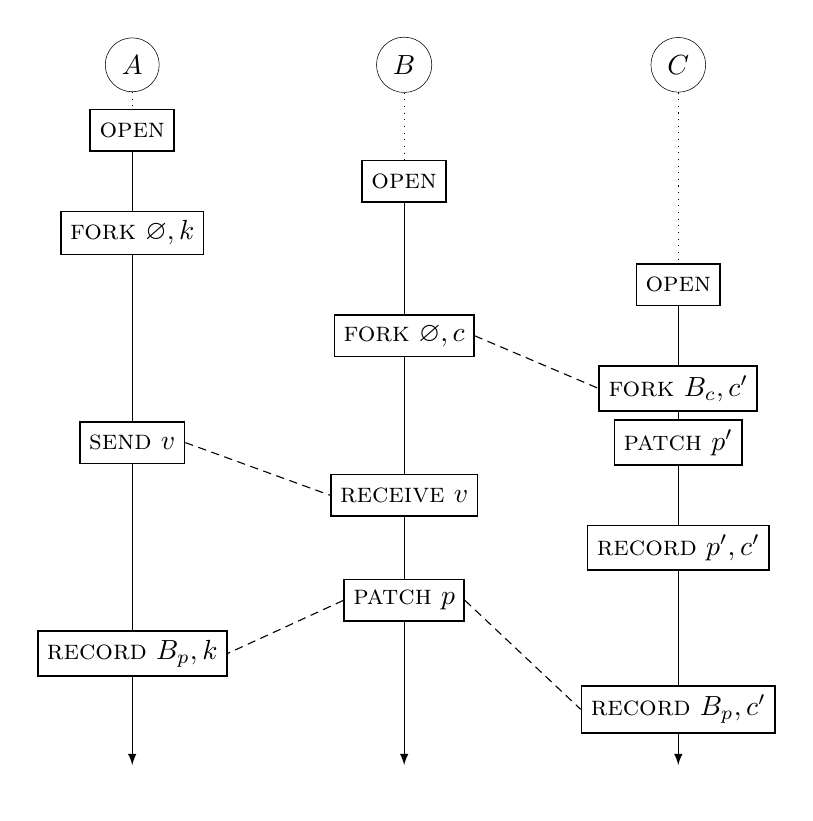
\begin{tikzpicture}
    \tikzstyle{link} = [-, thin, densely dashed];
    \tikzstyle{pointer} = [thin, -latex];
    \tikzstyle{account} = [draw, circle, font=\Small];
    \tikzstyle{tx} = [fill=white, rectangle, draw, semithick, minimum width=3em, minimum height=1.5em, font=\Small];
    \tikzstyle{end} = [];
    \tikzstyle{sync} = [-, densely dashed];

    \node [matrix, very thin, column sep=1.3cm, row sep=0.1cm] (matrix) at (0, 0) {
        \node[account] (A) {$A$};                         & \node[account] (B) {$B$};                         & \node[account] (C) {$C$};                    \\
                                                          &                                                   &                                              \\
        \node[tx] (A-open) {\textsc{open}};               &                                                   &                                              \\
                                                          & \node[tx] (B-open) {\textsc{open}};               &                                              \\
        \node[tx] (A-1) {\textsc{fork} $\varnothing, k$}; &                                                   &                                              \\
                                                          &                                                   & \node[tx] (C-open) {\textsc{open}};          \\
                                                          & \node[tx] (B-1) {\textsc{fork} $\varnothing, c$}; &                                              \\
                                                          &                                                   & \node[tx] (C-1) {\textsc{fork} $B_c, c'$};   \\
        \node[tx] (A-2) {\textsc{send} $v$};              &                                                   & \node[tx] (C-2) {\textsc{patch} $p'$};       \\
                                                          & \node[tx] (B-2) {\textsc{receive} $v$};           &                                              \\
                                                          &                                                   & \node[tx] (C-3) {\textsc{record} $p', c'$};  \\
                                                          & \node[tx] (B-3) {\textsc{patch} $p$};             &                                              \\
        \node[tx] (A-3) {\textsc{record} $B_p, k$};       &                                                   &                                              \\
                                                          &                                                   & \node[tx] (C-4) {\textsc{record} $B_p, c'$}; \\
                                                          &                                                   &                                              \\
                                                          &                                                   &                                              \\
                                                          &                                                   &                                              \\
        \node[end] (A-end) {};                            & \node[end] (B-end) {};                            & \node[end] (C-end) {};                       \\
    };

    \begin{scope}[on background layer]
        \draw[-, dotted] (B)        to (B-open);
        \draw[-, dotted] (C)        to (C-open);
        \draw[-, dotted] (A)        to (A-open);
        \draw[-latex]    (A-open)   to (A-end);
        \draw[-latex]    (B-open)   to (B-end);
        \draw[-latex]    (C-open)   to (C-end);
        \draw[sync]      (A-2.east) to (B-2.west);
        \draw[sync]      (B-1.east) to (C-1.west);
        \draw[sync]      (B-3.east) to (C-4.west);
        \draw[sync]      (B-3.west) to (A-3.east);
    \end{scope}
\end{tikzpicture}
\end{document}

    \captionof{figure}{Three accounts, $A$, $B$ and $C$, and their transaction chains.
        The diagram illustrates free transactions, such as \textsc{open} and
        \textsc{patch}, as well as dependent transactions such as \textsc{send}
        and \textsc{receive}.  The dashed lines represent cross-chain
        synchronizations between dependent transactions.
    \label{tx-dependencies}}
\end{fig}

\begin{description}
    \item[Send/Receive] $\tx{send}{s, r, v}_{\sigma}$ and
        $\tx{receive}{t_{id}}_{\sigma}$. Send $v$ tokens from $s$ to $r$. In
        order for the tokens to be claimed on the receiving account, the
        transaction hash $t_{id} = \hash(t)$ of the \textsc{send} transaction
        $t$ must be specified by \textsc{receive}.
    \item[Patch/Record] $\tx{patch}{p}_\sigma$ and $\tx{record}{t_{id},
        r_c}_{\sigma}$.  Add a patchset $p$ to the context $r_c$. The
        \textsc{patch} transaction $t$ adds a context-free patch $p$ to an
        account ledger $a$, without applying it. It can later be applied to a
        context $r_c$ in any account $a' \in \mathcal{A}$ (including $a$), by
        the \textsc{record} operation, which must reference the hash $t_{id} =
        \hash(t)$ of $t$.
        % TODO: Define patch in detail.
    \item[Fork] $\tx{fork}{k_c, k_{c'}}_\sigma \; \text{where} \; k_c \neq
        \mathcal{C}_{\varnothing}$. Create a new context $k_{c'}$ from an
        existing context $k_c$. Note that $k_c$ and $k_{c'}$ may belong to
        different accounts.
\end{description}

\subsubsection{Genesis State}
\subsubsection{Chain Growth}

\subsubsection{Git}
\subsubsection{Patch Theory}

\subsection{Consensus}
\label{consensus}

\subsubsection{Finality}
\label{finality}

\subsubsection{Sybil Resistance}
\label{sybil-resistance}


\end{multicols}

\appendix
\end{document}
